\documentclass[12pt]{article}

\usepackage{sbc-template}     % Modelo de relatório SBC
\usepackage[utf8]{inputenc}   % Codificação de entrada UTF-8
\usepackage[T1]{fontenc}      % Codificação de fonte: T1
\usepackage[brazil]{babel}    % Idioma português brasileiro
\usepackage{graphicx}         % Inclusão de imagens externas
\usepackage{minted}           % Destaque de sintaxe de código-fonte
\usepackage{caption}          % Legendas para imagens, tabelas, listagens, ...
\usepackage{hyperref}         % Referências em forma de links na saída em PDF

\title{Manipulador de Gramáticas Regulares e Livres de Contexto}

\author{Eduardo Weiland\inst{1}}
\address{Curso de Ciência da Computação -- Universidade de Santa Cruz do Sul (UNISC)\\
  Santa Cruz do Sul -- RS -- Brasil
  \email{eduardoweiland@mx2.unisc.br}
}

% ===========================================
% Configurações para listagens/código-fonte
% -------------------------------------------
\newcommand{\codefontsize}{\footnotesize}
\renewcommand\listingscaption{Listagem}
\providecommand*{\listingautorefname}{Listagem}

\newminted{js}{linenos,numbersep=5pt,frame=leftline,framesep=2mm,fontsize=\codefontsize}

% http://tex.stackexchange.com/questions/12428/code-spanning-over-two-pages-with-minted-inside-listing-with-caption
\newenvironment{code}{\captionsetup{type=listing}}{}

% ===========================================
% Configurações de links na saída em PDF
% -------------------------------------------
\hypersetup{
  pdftitle={Manipulador de Gramáticas Regulares e Livres de Contexto},
  pdfauthor={Eduardo Weiland},
  pdfcreator={\LaTeX},
  pdfsubject={Manipulador de Gramáticas Regulares e Livres de Contexto (Trabalho de Linguagens Formais UNISC 2015/1)},
  pdfproducer={LaTeX},
  colorlinks=true,
  linkcolor=blue,
  citecolor=blue,
  filecolor=blue,
  urlcolor=blue,
  bookmarksdepth=4
}

\begin{document}

\maketitle

\begin{resumo}
  Este artigo relata as etapas do desenvolvimento de uma ferramenta para manipulação de gramáticas regulares e livres
  de contexto, desenvolvido na disciplina de Linguagens Formais da Universidade de Santa Cruz do Sul, no primeiro
  semestre de 2015.
\end{resumo}

%%%%%%%%%%%%%%%%%%%%%%%%%%%%%%%%%%%%%%%%%%%%%%%%%%%%%%%%%%%%%%%%%%%%%%%%%%%%%%%%%%%%%%%%%%%%%%%%%%%%%%%%%%%%%%%%%%%%%%%%

\section{Manipulador de Gramáticas}

Este artigo relata o processo de desenvolvimento de uma ferramenta para manipulação de gramáticas regulares e livres de
contexto. Essa ferramenta é um trabalho desenvolvido na disciplina de Linguagens Formais na Universidade de Santa Cruz
do Sul.

O ferramenta é dividida em duas partes: a primeira delas consiste em uma interface que permite criar interativamente
uma gramática do tipo regular ou do tipo livre de contexto; a segunda parte é um reconhecedor do tipo autômato finito
determinístico, capaz de reconhecer sentenças a partir de uma definição inicial.

O manipulador de gramática deve permitir a entrada de uma gramática qualquer pelo usuário, através de campos para a
definição dos símbolos não terminais e terminais, o símbolo de início de produção e todo o conjunto de produções. A
partir dessas entradas, é esperado que o programa verifique se a gramática entrada é válida, exiba o seu formalismo,
classifique-a na hierarquia de Chomsky e gere automaticamente duas sentenças para essa gramática.

O autômato finito que atua como reconhecedor deve ser representado através de uma tabela de transição de estados, que
deve ser editável. Nesta tabela são definidos os símbolos reconheciso pelo autômato e os estados utilizados durante o
reconhecimento, bem como todas as regras de leitura dos símbolos e definição do próximo estado. O autômato deve
demonstrar passo-a-passo o processo de reconhecimento das sentenças informadas pelo usuário.

%%%%%%%%%%%%%%%%%%%%%%%%%%%%%%%%%%%%%%%%%%%%%%%%%%%%%%%%%%%%%%%%%%%%%%%%%%%%%%%%%%%%%%%%%%%%%%%%%%%%%%%%%%%%%%%%%%%%%%%%

\section{Desenvolvimento}

A ferramenta foi desenvolvida como uma aplicação \textit{web} executada totalmente no lado cliente (\textit{clientside}).
Para isso, foi utilizada a linguagem de programação JavaScript em conjunto com algumas bibliotecas e outras ferramentas
de uso livre para facilitar a organização e a programação do trabalho.

\subsection{Estrutura}

Para gerenciar as bibliotecas de terceiros, foram utilizadas as ferramentas \textit{npm} \cite{npm} e \textit{bower}
\cite{bower}. O primeiro deles é utilizado principalmente para algumas ferramentas utilizadas apenas durante o
desenvolvimento, incluindo o próprio \texttt{bower}. Este, por sua vez, é responsável por gerenciar as dependências
das bibliotecas que são realmente utilizadas no trabalho.

O uso dessas ferramentas permite apenas descrever quais versões de quais bibliotecas são necessárias, e a partir dessa
configuração tudo pode ser instalado em apenas um comando: \texttt{npm install}. Após a execução desse comando, é
necessário apenas publicar os arquivos do projeto em algum servidor HTTP e, em seguida, acessar o projeto utilizando
algum navegador \textit{web} moderno.

A versão estável mais recente do trabalho está disponível para acesso livre em um servidor \textit{online}, sem a
necessidade de realizar a instalação de outras ferramentas e dependências. O \textit{link} para acessá-la é
\href{https://eduardoweiland.github.io/manipulador-gramaticas}{https://eduardoweiland.github.io/manipulador-gramaticas}.

\subsection{Organização do Projeto}

O código fonte desenvolvido nesse trabalho está localizado dentro do diretório \texttt{app} na raiz do projeto. Neste
deste diretório, o arquivo \texttt{index.html} e o subdiretório \texttt{css} são responsáveis apenas pela apresentação
dos resultados na tela. A lógica da execução está toda implementada nos arquivos localizado dentro da pasta \texttt{js}.

A ligação entre a exibição dos dados na interface e a lógica da ferramente é feita pela ferramenta Knockout
\cite{knockout}. Essa ferramenta é parte importante do \textit{software} desenvolvido, visto que é a ferramenta que
centraliza a entrada de dados por parte do usuário e a exibição dos resultados, tudo gerenciado de forma automática.

A implementação do trabalho foi dividida em diversas classes, cada uma delas responsáveis por realizar alguma tarefa
específica pré-determinada. A integração destas classes é feita primariamente utilizando referências para instâncias
das outras classes em propriedades do objeto em questão.

Foram criadas quatro classes para representar as diversas ramificações existentes para a execução da tarefa designada
para este trabalho. São elas:

\begin{description}
  \item[ProductionRule]
  Representação de uma única regra de produção que compõe a gramática à qual a regra pertence. Não depende diretamente
  de outras classes, no entanto recebe por parâmetro no construtor uma referência para a gramática da qual é parte
  integrante, utilizando-se dessa referência para acessar algumas informações relevantes às suas atribuições.

  \item[Grammar]
  Responsável pelas tarefas de mais alto nível dentro da criação da gramática, validação, classificação e geração de
  sentenças. Depende exclusivamente da classe ProductionRule.

  \item[TransitionTable]
  É a classe que implementa as tarefas mais básicas para a edição e o funcionamento geral de autômato finito. Armazena
  internamente todas as definição da tabela de transição de estados informadas pelo usuário na interface do
  \textit{software} desenvolvido, sendo referência para a implementação da lógica de reconhecimento do autômato.

  \item[FiniteAutomaton]
  Implementa a funcionalidade de leitura de uma sentença e reconhecimento da mesma, armazenando todas as etapas executadas
  para que sejam exibidas na interface, caso o reconhecimento seja executado com êxito.
\end{description}

Essas classes foram implementadas no formato de módulos para o RequireJS, uma das bibliotecas que foram utilizadas no
\textit{software}, que é responsável por gerenciar as dependências entre os módulos e o carregamento assíncrono dos
arquivos quando necessário. Um exemplo de como um módulo do RequireJS é definido é exibido na \autoref{lst:modulo-rjs}

\begin{code}
  \caption{Exemplo de definição de módulo do RequireJS}
  \label{lst:modulo-rjs}
  \begin{jscode}
define(['knockout'], function(ko) {
    'use strict';

    // ...

    function TransitionTable() {
        this.init.apply(this, arguments);
    }

    // ...

    return TransitionTable;
});
  \end{jscode}
\end{code}

O módulo definido na \autoref{lst:modulo-rjs} pode ser utilizado em outros módulos apenas referenciando o nome do
arquivo em que ele está implementado. Desta forma, é possível manter o código-fonte melhor organizado e modular,
facilitando o entendimento do mesmo.

Nenhuma das classes desenvolvidas utiliza herança, visto que o sistema é muito específico e, dessa forma, não há
vantagens significativas em criar generalizações para os objetos manipulados. Assim sendo, todos os módulos definem
uma classe com seus devidos atributos e os métodos adicionados ao protótipo e, por fim, apenas exportam o construtor
desta classe.

As dependências necessárias são integradas utilizando a técnica de composição, sendo que assim uma referência a um
objeto que é dependência poderá ser exportada juntamente ao módulos, mas seu construtor não será exposto externamente,
mantendo o isolamento entre os diversos componentes do \textit{software}. Ou seja, por exemplo, quem instanciar um
objeto da classe \texttt{Grammar} não precisa atentar para o fato de que um objeto do tipo \texttt{ProductionRule} é
utilizado para auxiliar nas tarefas necessárias.

\subsection{Observáveis}

Uma das principais funcionalidades oferecidas pelo Knockout \cite{knockout} é o conceito de \textit{observables}, ou
observáveis. Essa ideia consiste de objetos JavaScript que podem ser associados a elementos no \texttt{DOM} e a
biblioteca se responsabiliza por atualizar os valores tanto das variáveis no JavaScript quanto dos elementos no
\texttt{DOM} todas as vezes que ocorre alguma modificação do valor de forma automática.

Essa técnica também é conhecida como \textit{two-way binding}, ou ligação de duas vias. Com isso, quando um campo de
entrada de texto é "ligado" a uma variável string no JavaScript, por exemplo, todas as vezes que a variável for
modificada programaticamente, essas modificações também serão visíveis no campo da tela. O contrário funciona da mesma
forma, sendo que todas as vezes que o usuário modificar o valor do campo na interface, a variável no JavaScript será
atualizada.

Outra vantagem introduzida pelo Knockout são os valores computados (\textit{computed}). São valores que, como o nome
sugere, são calculados a partir de outros dados. Geralmente, esses dados também são observáveis, e, nesses casos, os
valores computados também são recalculados todas as vezes que um observável do qual ele depende é atualizado.

\subsection{Interface}

A interface do usuário foi desenvolvida utilizando-se a biblioteca Bootstrap \cite{bootstrap}. O Bootstrap é formado
por diversos componentes que permitem criar uma interface \textit{web} adaptada a diversas resoluções de tela
(\textit{design} responsivo) de forma simples e rápida.

A página do \textit{software}, ao ser aberta, apresenta duas abas, sendo que a primeira delas já se encontra selecionada.
Essas duas abas permitem acessar as duas partes do trabalho desenvolvido, e, em cada uma delas, preencher as informações
necessárias e visualizar todos os resultados gerados sem a necessidade de novas interações para que eles sejam visíveis.
Isto é, no momento em que os dados de entrada são inseridos no software, se estes já forem suficientes para processar e
gerar um resultado, isso já será feito automaticamente.

\begin{figure}[ht]
  \centering
  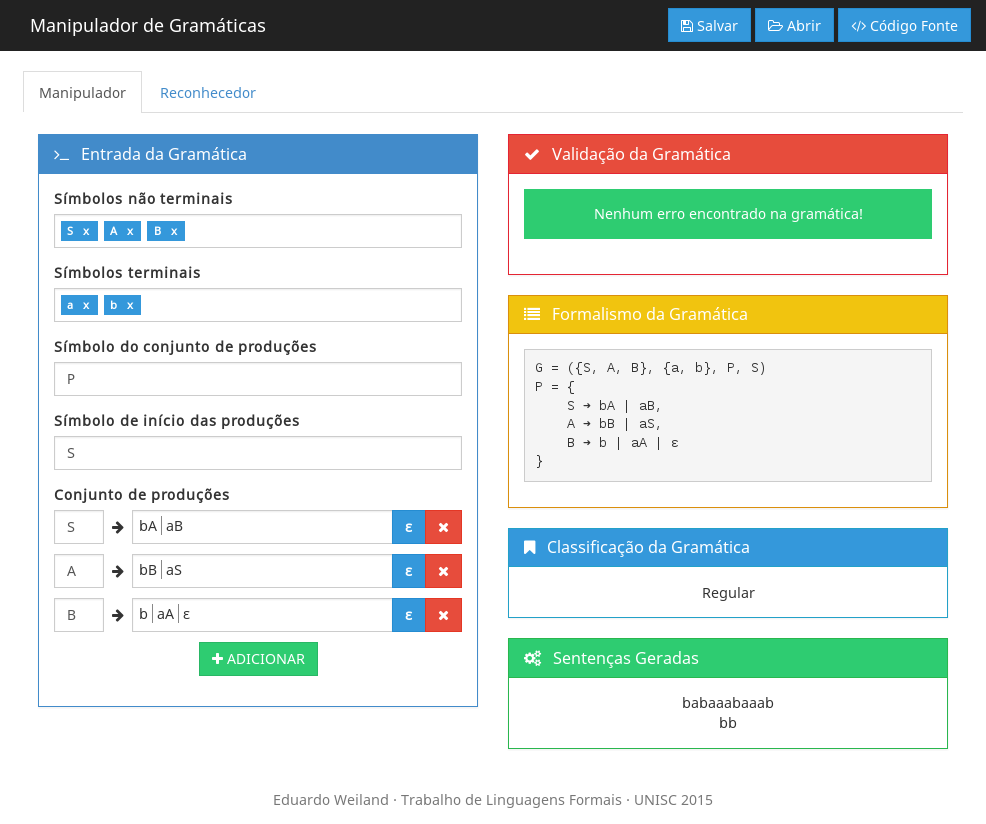
\includegraphics[width=\textwidth]{images/manipulador.png}
  \caption{Tela principal do manipulador de gramáticas}
  \label{fig:manipulador}
\end{figure}

Na \autoref{fig:manipulador}, é exibida a interface inicial do software que é também a tela principal do manipulador
de gramáticas. Nessa interface as gramáticas são construídas pelo usuário de forma intuitiva a partir do preenchimento
dos campos do lado esquerdo da tela, e do lado direito são exibidos os resultados obtidos da análise da gramática criada.

\begin{figure}[ht]
  \centering
  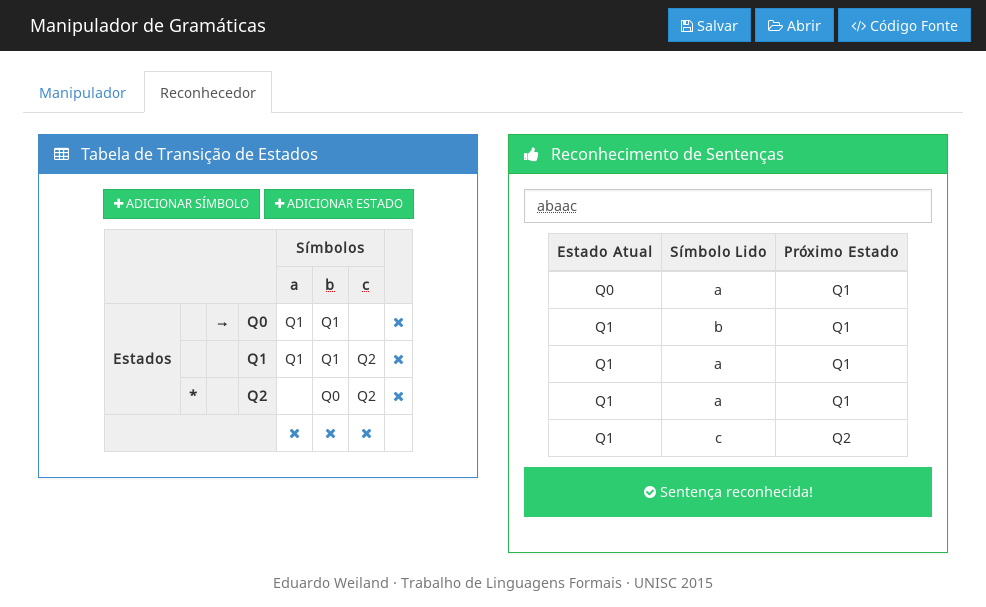
\includegraphics[width=\textwidth]{images/reconhecedor.png}
  \caption{Tela com o autômato finito e o reconhecimento de uma sentença}
  \label{fig:reconhecedor}
\end{figure}

Já na \autoref{fig:reconhecedor}, pode-se ver a segunda aba do sistema que é a interface do autômato finito, representado
através de uma tabela de transição de estados editável do lado esquerdo da tela. O lado direito, novamente, é onde os
resultados são exibidos, nesse caso, as etapas de reconhecimento de uma sentença.

%%%%%%%%%%%%%%%%%%%%%%%%%%%%%%%%%%%%%%%%%%%%%%%%%%%%%%%%%%%%%%%%%%%%%%%%%%%%%%%%%%%%%%%%%%%%%%%%%%%%%%%%%%%%%%%%%%%%%%%%

\bibliographystyle{abbrv}
\bibliography{report}

%%%%%%%%%%%%%%%%%%%%%%%%%%%%%%%%%%%%%%%%%%%%%%%%%%%%%%%%%%%%%%%%%%%%%%%%%%%%%%%%%%%%%%%%%%%%%%%%%%%%%%%%%%%%%%%%%%%%%%%%

\end{document}
